\begin{center}
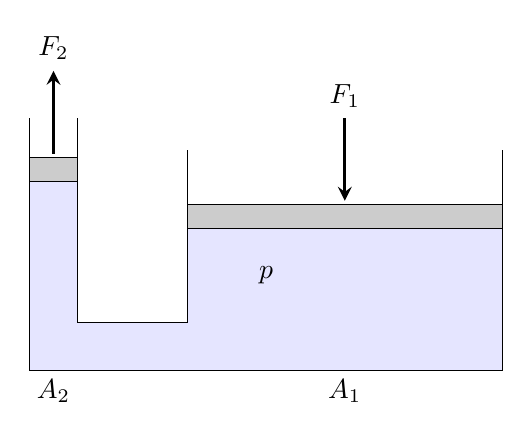
\begin{tikzpicture}[>=stealth]
 \fill[blue!10] (0,0) rectangle (6,0.6);
 \fill[blue!10] (0,0.6) rectangle (0.6,2.4);
 \fill[blue!10] (2,0.6) rectangle (6,1.8);
 \draw (0,3.2) -- (0,0) -- (6,0) -- (6,2.8);
 \draw (0.6,3.2) -- (0.6,0.6) -- (2,0.6) -- (2,2.8);
 \draw[fill=gray!40] (0,2.4) rectangle (0.6,2.7);
 \draw[fill=gray!40] (2,1.8) rectangle (6,2.1);
 \draw[->, very thick] (0.3,2.75) -- (0.3,3.8) node[above] {$F_2$};
 \draw[->, very thick] (4,3.2) -- (4,2.15) node[pos=0, above] {$F_1$};
 \node[below] at (0.3,0) {$A_2$};
 \node[below] at (4,0) {$A_1$};
 \node at (3,1.2) {$p$};
\end{tikzpicture}
\end{center}

Der Kolben im grossen Zylinder (Fläche $A_1$) erzeugt in der Flüssigkeit den Druck $p = F_1/A_1$. Dieser Druck ist überall in der Flüssigkeit gleich und drückt auf den kleinen Kolben (Fläche $A_2$) mit der Kraft
\begin{align}
 F_2 &= p\,A_2 = \FzkF \\
   &= \frac{1}{\vzy}\cdot\Fzg \\
   &= \Fzk \approx \result{\FzkP{0}{2}}
\end{align}
Um den kleinen Kolben festzuhalten, braucht es also nur einen Drittel der Kraft.
